\documentclass{article}
\usepackage{graphicx}
\usepackage{hyperref}
\hypersetup{%
	pdfborder = {0 0 0 0}
}
\title{CS211 Class Description}
\date{2013-05-02}
\author{Christopher Marriott, cpm4@aber.ac.uk}

\begin{document}
\maketitle
\newpage
\tableofcontents
\newpage

\section{Brief description of scheduler classes}
Each scheduler class implements the scheduler interface. The interface has six methods defined. These are, getNextJob, addNewJob, returnJob, removeJob, reset and getJobList. 

\section{First come first serve class}
This class implements the scheduler interface and uses all but the returnJob functions. This just passes the head of the queue back to be processed.

\section{Highest Priority Class}
This class implements the scheduler interface and makes use of all methods. The highest priority job is placed at the front on the cue when adding and removing.

\section{Shortest time first class}
This class implements the scheduler interface and uses all methods. This class will do the same as highest priority class but with the shortest length going to the head of the queue rather than the highest priority.

\section{Round robin}
This class implements the scheduler interface and uses all methods. This class allocates a time portion to each process at the head of the queue, when that time is used up it goes to the back of the queue.

\section{High response ration next}
This class implements the scheduler interface and uses all methods. This class takes into account the length of the job and the time it has been waiting in the queue. It then calculates the new priority and puts the job with the highest priority at the head od the queue.


\section{Classes}
Key: 
\begin{itemize}
	\item Yellow Diamond = Protected
	\item Red Square = Private
	\item Green circle = method
	\item Green circle with C = Constructor
\end{itemize}
\begin{center}
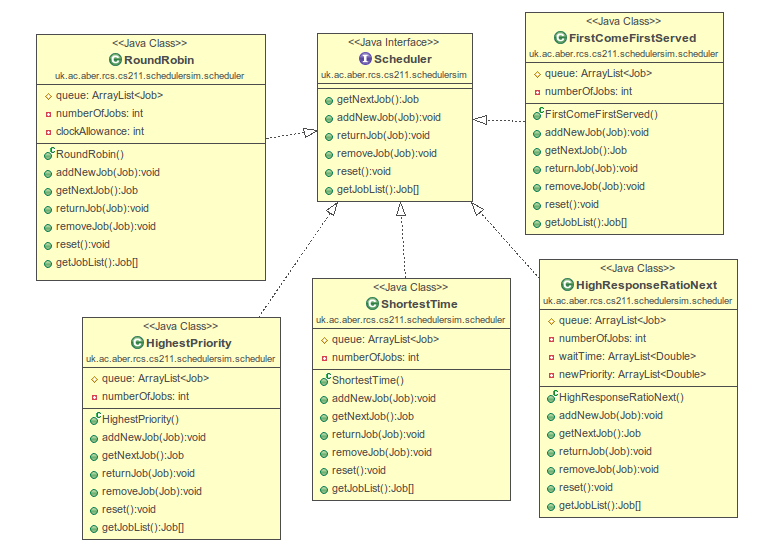
\includegraphics[scale=0.6]{class.png}
\end{center}


\end{document}

